%%%%%%%%%%%%%%%%%%%%%%%%%%%%%%%%%%%%%%%%%
% University Assignment Title Page 
% LaTeX Template
% Version 1.0 (27/12/12)
%
% This template has been downloaded from:
% http://www.LaTeXTemplates.com
%
% Original author:
% WikiBooks (http://en.wikibooks.org/wiki/LaTeX/Title_Creation)
%
% License:
% CC BY-NC-SA 3.0 (http://creativecommons.org/licenses/by-nc-sa/3.0/)
% 
% Instructions for using this template:
% This title page is capable of being compiled as is. This is not useful for 
% including it in another document. To do this, you have two options: 
%
% 1) Copy/paste everything between \begin{document} and \end{document} 
% starting at \begin{titlepage} and paste this into another LaTeX file where you 
% want your title page.
% OR
% 2) Remove everything outside the \begin{titlepage} and \end{titlepage} and 
% move this file to the same directory as the LaTeX file you wish to add it to. 
% Then add \input{./title_page_1.tex} to your LaTeX file where you want your
% title page.
%
%%%%%%%%%%%%%%%%%%%%%%%%%%%%%%%%%%%%%%%%%
%\title{Title page with logo}
%----------------------------------------------------------------------------------------
%	PACKAGES AND OTHER DOCUMENT CONFIGURATIONS
%----------------------------------------------------------------------------------------

\documentclass[12pt]{article}
\usepackage[english]{babel}
\usepackage[utf8x]{inputenc}
\usepackage{amsmath}
\usepackage{graphicx}
\usepackage{subcaption}
\usepackage{float}
\usepackage[colorinlistoftodos]{todonotes}
\usepackage{hyperref}
\usepackage{algorithm2e}



\textheight=230truemm 
\textwidth=160truemm 
\hoffset=-10truemm \voffset=-20truemm

\begin{document}

\begin{titlepage}

\newcommand{\HRule}{\rule{\linewidth}{0.5mm}} % Defines a new command for the horizontal lines, change thickness here

\center % Center everything on the page
 
%----------------------------------------------------------------------------------------
%	HEADING SECTIONS
%----------------------------------------------------------------------------------------

\textsc{\LARGE Ukrainian Catholic University}\\[1cm] % Name of your university/college
\textsc{\Large  Faculty of Applied Sciences}\\[0.5cm] % Major heading such as course name
\textsc{\large Data Science Master Programme}\\[0.5cm] % Minor heading such as course title

%----------------------------------------------------------------------------------------
%	TITLE SECTION
%----------------------------------------------------------------------------------------
\vspace*{1cm}

\HRule \\[0.4cm]
{ \huge \bfseries Facial Expression Recognition in Natural Images}\\[10pt]
{\Large \bfseries Machine Learning final project progress report}\\[0.4cm] % Title of your document
\HRule \\[1cm]
 
%----------------------------------------------------------------------------------------
%	AUTHOR SECTION
%----------------------------------------------------------------------------------------
\vspace*{1cm}

% If you don't want a supervisor, uncomment the two lines below and remove the section above
\Large \emph{Authors:}\\
Anastasiia \textsc{Khaburska}\\Andrii \textsc{Yurkiv}\\[1cm] % Your name

%----------------------------------------------------------------------------------------
%	DATE SECTION
%----------------------------------------------------------------------------------------
\vspace*{1cm}
{\large 27 April 2019}\\[2cm] % Date, change the \today to a set date if you want to be precise

%----------------------------------------------------------------------------------------
%	LOGO SECTION
%----------------------------------------------------------------------------------------

\includegraphics[height=5cm]{UCU-Apps.png}\\[1cm] % Include a department/university logo - this will require the graphicx package
 
%----------------------------------------------------------------------------------------

\vfill % Fill the rest of the page with whitespace

\end{titlepage}


% \begin{abstract}
	
% \end{abstract}

\section{Introduction}

Facial expression is one or more motions or positions of the muscles beneath the skin of the face. These movements convey the emotional state of an individual and become the primal form of nonverbal communication.\\

It is assumed that certain facial expressions and gestures correspond to specific emotions (for instance, happiness is associated with laughter and smiling, sadness with tears, anger with clenched jaw, fear with grimace, surprise with raised eyebrows and wide eyes and disgust with wrinkled nose and squinted eyes) which  are recognized by humans regardless of culture, language or time. But in general, this hypothesis has not been scientifically verified and received both critical and supportive reviews.\\

Both sides of this scientific debate agree that the face expresses emotion. The controversy surrounds the uncertainty about what specific emotional information is read from a facial expression \cite{wiki}.


\section{Motivation}

It has been proved multiple times that the majority of information human perceives (up to $83\%$) during message absorption is obtained through eyesight. For this purpose body language in general, and facial expression, in particular, are the things which provide the most essential and specific information about the intentions and emotional state of the message source.\\

It's not hard to conclude that accurate perception of facial expressions is a key to effective face-to-face communication.\\

Humans have a great ability to perform this kind of tasks. And since main facial expressions are universal and do not vary with culture or environment, we usually recognize others emotional state pretty well (at least when our interlocutors are not intentionally hiding it).\\

But for a machine, it is not an easy task. There are few reasons why machine learning model usually perform much worse compared to humans in recognizing facial expressions (while outperforming in other classification tasks):
\begin{itemize}
    \item 
    Humans do not perceive facial expressions separately from other parts of body language. For facial expressions, context is very important, because it provides a great deal of additional information.
    \item
    Regardless of their universality, facial expressions are very diverse and vary substantially due to the race, age, gender, nationality and culture.
    \item 
    People are brilliant at determining how they feel. But in some cultures, it is normal to hide your real emotions behind the neutral or happy facial expression. It is especially distinguishable in western cultures, where excessive emotionality is not considered as an element of effective communication. Machine learning model doesn't have this prior knowledge and hence use a generalized approach to cases where cultural nuances are crucial.
    \item 
    Some kinds of facial expressions are very similar (for example, without context, it's hard to distinguish surprise from fear, or sadness from neutrality). And image similarity is a fundamental property when the model is trying to determine class depicted on it. The model fails to generalize well and makes mistakes by focusing on the wrong features.
\end{itemize}

In this project, we investigated deep learning aproaches to the task of facial expression recognition and  developed an end-to-end machine learning system of facial expression recognition in natural images. It consists of two parts: a face detector and expression recognizer. Unfortunately, we haven't found a data set to evaluate our end-to-end system (we need a data set that contains images with faced in different contexts labelled with facial expression classes). So, we evaluated our results in conjunction with state-of-the-art performance on \texttt{fer2013} data set, which is equal to $75.2\%$

\section{Project idea. Data}

The project idea was inspired by Kaggle competition "Challenges in Representation Learning: Facial Expression Recognition Challenge". It was organized in 2013, but we think that the topic is still relevant today. The \texttt{fer2013} data set \cite{dataset} for this competition was prepared by Pierre-Luc Carrier and Aaron Courville.\\

The \texttt{fer2013} data set consists of $48\times48$ pixel gray-scale images of faces. The faces have been automatically registered so that the face is more or less centered and occupies about the same amount of space in each image. The task is to categorize each face based on the emotion shown in the facial expression into one of seven categories (0=Angry, 1=Disgust, 2=Fear, 3=Happy, 4=Sad, 5=Surprise, 6=Neutral).\\

The data set is divided into train, validation and test splits. The training set consists of $28,709$ examples. The validation set consists of $3,589$ examples. The final test set consists of another $3,589$ examples.\\

\begin{table}[H]
	\centering
	\begin{tabular}{ | l | l | l | l | l | }
		\hline
		Expression & Train & Validation & Test & \% of samples \\ \hline
		Angry & 3995 & 467 & 491 & 13.8 \\ %\hline
		Disgust & 436 & 56 & 55 & \textbf{1.52} \\ %\hline
		Fear & 4097 & 496 & 528 & 14.27 \\ %\hline
		Happy & 7215 & 895 & 879 & \textbf{25.05} \\ %\hline
		Neutral & 4965 & 607 & 626 & 17.27 \\ %\hline
		Sad & 4830 & 653 & 594 & 16.93 \\ %\hline
		Surprise & 3171 & 415 & 416 & 11.15 \\ 
		\hline
	\end{tabular}
	\caption{Distribution of classes in the data set.}
\end{table}

The classes in the data set are not well-balanced. First of all, we have highly underrepresented \texttt{Disgust} class. Also, $25.05\%$ of samples correspond to the \texttt{Happy} class, which is more than the fraction of \texttt{Angry} and \texttt{Surprise} altogether ($24.95\%$).\\ 

This imbalance issue imposes additional activities in our development process:

\begin{itemize}
    \item 
    We performed data augmentation in order to make it more robust.
    \item
    We used minibatch normalization, to reduse the covarianse shift and to increase training rates.
    \item
    As an evaluation metric, we used the confusion matrix to determine the weaknesses of the model and possible improvement strategies.
\end{itemize}

Besides the imbalance, \texttt{fer2013} data set contains trash samples (which do not contain a face) and several misclassified examples. These imperfections make the classification harder because the model has to generalise well and be robust to incorrect data. To adress this problem and clean the dataset we used our first part of solution -- face recognition.

\section{Approach to the solution}
\subsection{Baseline model}


At this point, for face detection we are using pretrained Haar Cascade model from \texttt{cv2} python module. Since we don't have a data set on which we can assess both face detection and facial recognition models performance, we would not concentrate on it's implementation in this part.\\

In the next iteration, to make our pipeline more homogeneous, we are going to implement and train our own model for face detection.\\

Our baseline facial expression recognition model is a 4-layer CNN with 3 dense layers. The model architecture is visualized in figure 1.\\

On each layer except output one we used ReLU activation function. On the output layer we used Softmax function. Besides it, we applied the Dropout regularization technique at each layer of our model because otherwise it didn't train properly and stuck in the local minima. \\

The details of implementation can be viewed in corresponding jupyter notebook: (\texttt{classification.ipynb}).\\

\begin{figure}
	\centering
	\includegraphics[width=\textwidth]{../images/baseline-architecture.png}
	\caption{Baseline CNN model}
\end{figure}

You can find the example of model results in figure 2 in the Appendix.
\subsection{VGG}
\subsection{Dropout}
\subsection{Batch normalization}
\subsection{Ensamble}

\section{Evaluation}

Our baseline model gave $63.25\%$ accuracy on the test dataset. In the original competition leaderboard, it would be in the top 10 submissions. We think that it is possible to get even higher accuracy by training the model for larger number of epochs. Still, it is only a baseline model, and in the future iteration we are going to improve this result.\\ 

During the data analysis stage of our project, we understood that one of the primary weaknesses of this data set is its imbalance. We haven't tackled this issue yet (plan to do it in the next iteration), but we understood that dealing with it is a major part of this particular problem solution.\\

The thing is that during the evaluation stage we've got very unexpected results. \texttt{Disgust} emotion while being extremely underrepresented in our data set is not the one that suffers most from misclassification. It is \texttt{Angry} and \texttt{Fear}, that model most often treats as other facial expression.\\

\texttt{Fear} is mostly confused with  \texttt{Sad}. Maybe because often when a person experiences fear, it doesn't influence her facial expression and has an impact only on some inner feelings. In general, when we are afraid of something, we can have different facial expression, depending on the situation, surrounding and the cause of fear. Fear is a complex emotion no single facial expression corresponds to it.\\

From the confusion matrix, we can conclude 3 out of 6 facial expressions are often confused with \texttt{Sad}. It looks like this is the most obvious way for the model to describe the appearance if it is not sure what it sees.\\

One important thing should be noted here: the results produced by our the model does not confirm our primary assumption that accuracy of classification of images will be smaller for underrepresented classes. It proves one more time that the problem of facial expression recognition is not as simple as it seems from the first sight.

\begin{figure}
	\centering
	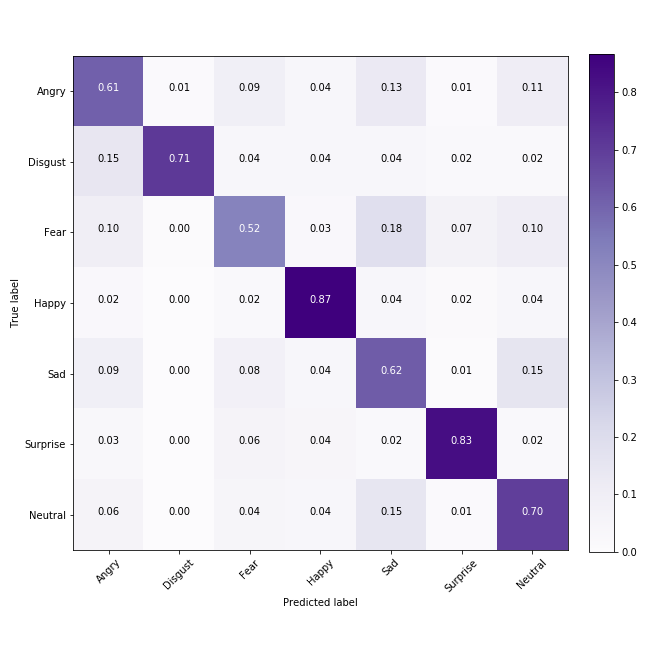
\includegraphics[width=0.65\textwidth]{../images/confusion.png}
	\caption{Normalized confusion matrix}
\end{figure}

\section{Comparisons}

\section{Conclusions}

We plan to do the following steps during the next iterations:

\begin{itemize}
	\item 
	Perform data augmentation for underrepresented classes and check whether it improves the results.
	\item 
	Apply other CNN architecture to this problem: VGG, Inception, ResNet.
	\item 
	Increase number of features by adding Face Landmarks and HOG.
	\item 
	Write script for facial expression recognition in videos.
	\item 
	Perform some basic hyperparameter tuning (model is complex, so it's complicated to iterate fast).
	\item 
	Try to solve misclassification problem for \texttt{Angry} and \texttt{Fear} classes.
\end{itemize}


\newpage
\begin{thebibliography}{6}
	\bibitem{dataset} 
	I. Goodfellow et al.
	\textit{Challenges in Representation Learning: A report on three machine learning
		contests}. 
	arXiv, 2013
	\bibitem{wiki}
	Wikipedia contributors
	\textit{Facial expression}
	\href{https://en.wikipedia.org/wiki/Facial_expression}{Facial expression}
	


\end{thebibliography}

\newpage
\appendix
\section{Appendix}

\begin{figure}[h]
	\centering
	\begin{subfigure}[h]{0.65\textwidth}
		\includegraphics[width=\textwidth]{../data/original/test2.jpg}
		\caption{Original image}
	\end{subfigure}\qquad
	\begin{subfigure}[h]{0.65\textwidth}
		\includegraphics[width=\textwidth]{../images/test2_labeled.jpg}
		\caption{Predicted facial expressions}
	\end{subfigure}
	\caption{Baseline model results}
\end{figure}


\end{document}